
%FEHLT: 
% Biogenese eukaryotische RNA
% die 3 lacZ Standardfragen
% Qualitative, Quantitative Bestimmung von Molekülen in Gewebeschnitten
% Bioinformatische Suche nach kodierenden Gen Regionen (genau wie in Musterlösung) = Wie Gen/Expressionsort anhand von Nukleotidsequenz/Proteinsequenz finden, bioinformatisch
% mRNA seq in Prokaryioten die rRNA rausbekommen (genauer)
% MRI: Bauteile & Funktionsweise
% Promotor & Umgebung: Zeichnung beschriften
% Beschriftung DNA <-> RNA -> Protein -> Metabolit
% Enzymfunktion: Alkalische Phosphatase, Endonuklease, Polynukleotidkinase, reverse Transkriptase, Exonuklease, Taq-Polymerase
% Bakterielle rRNA-Anreicherung; tierisches Gewebe -> Genexpression qualitativ und quantitativ bestimmen mithilfe von RNA -> wie gehen Sie vor?
%%%% Relevante Sachen aus dem Praktikum !!
% mRNA-Sequenzierung
% Fragen von Nickis Protokollen
 
\section{Definitionen}
\testhead{Epigenetik}%3 
\testhead{Nukleotid}%1
\testhead{Lebendtiter}%p
\testhead{PMF}%10
\testhead{Metabolit}%11
\testhead{Nukleosom}%3
\testhead{Riboswitch}%8
\testhead{monoklonale und polyklonale Antikörper}
\testhead{Operon}%8
\testhead{Regulon}%8
\testhead{Stimulon}%8
\testhead{Replikon}%2
\testhead{Transposon}%3 %prak
\testhead{Disruptionsvektor}
\testhead{Synthenie}%6
\testhead{Genetischer Fingerabdruck}%prak


\section{Unterschiede}
\testhead{Unterschied zwischen miRNA und siRNA}%9
\testhead{Unterschied Illumina vs. Nanopore}%4
\testhead{Unterschied von BLAST und Smith-(Waterman-Algorithmus?) erklären}%7

\section{Beschreiben und Erklären}
\testhead{Welche Rolle spielen die Transkriptionsfaktoren bei Operon, Regulon u. Stimulon?}%8
\testhead{Beschreiben Sie Gen Assembly}%7
\testhead{Welche Probleme können bei Gen Assembly auftreten?}%7
\testhead{Wie bestimmt man einen Lebendtiter? (ausführlich)}%p
\testhead{Wie erhält man PMF und was stellt es dar?}%10
\testhead{Erklären Sie Illuma Sequencing}%4
\testhead{Definieren Sie die Mutationstypen}%prak
\testhead{Wie schützen sich Bakterien vor fremder DNA?}%prak
\testhead{Beschreiben Sie die Eigenschaften von Restriktionsendonuklease II}%p
\testhead{Welche Eigenschaften muss ein Vektor für tn5 Mutagenese auf jeden Fall aufweisen?}%p
\testhead{Zu welcher Transposon-Klasse gehört Tn5?}%prak
\testhead{Wofür codiert das Lacz-Gen?}%prak
\testhead{Welchen Nutzen und welche Funktion hat das Lacz-Gen in der Genomik?}%prak
\testhead{Wie kann man Metabolite qualitativ u. quantitativ in verschiedenen Regionen untersuchen?}%11
\testhead{Wie funktioniert qPCR, was ist der Ct-Wert und welche mRNA liegt am meisten vor?}%9
\testhead{Was ist iPCR? Erkläre das Prinzip.}
\testhead{Wie funktioniert ein Western Blot?}
\testhead{Was ist ein Massenspektrometer/Massenspektrometrie?}%11
\testhead{Chromatographie, welche gibt es, welche Eigenschaften müssen die Analyten haben und wie werden sie eluiert?}%11 
\testhead{Metabolitenbestimmung – allgemeiner Ablauf}%11
\testhead{Chromosomale DNA-Extraktion - allgemeiner Ablauf}%prak
\testhead{Wieso ist BLAST schneller als das Alignment nach W.?}%7
\testhead{Wodurch zeichnen sich bakterielle HFR-Stämme aus?}%2
\testhead{Wie entstehen bakterielle HFR-Stämme?}%2
\testhead{Worin unterscheiden sich unterschiedliche HFR-Stämme?}%2
\testhead{Wofür werden HFR-Stämme verwendet?}%2
\testhead{Was ist MALDI-Imaging und was wird damit dargestellt?}%11
\testhead{Was ist Southern Blot? Erkläre das Prinzip.}
\testhead{Was sind die Vorteile langer Reads?}%4
\testhead{Was sind die Nachteile von Oxford Nanopore?}%4
\testhead{Erklären sie die wichtigsten bestandteile von Souther Hybridisierung}%
\testhead{Was ist PACBIO-SMRT-Sequencing?}%4
\testhead{Eigenschaften für Vektoren mit large-insert Klonen. Nennen sie zwei Beispiele.}%5
\testhead{Welcher Schritt ist ausschlaggebend für die Pyrosequenzierung? In welchem Schritt wird detektiert?}%4
\testhead{Beschreiben sie die Isolierung von Plasmid-DNA}%2
\testhead{Ablauf einer Klonierung}%2
\head{Was ist ein SuicidePlasmid und wofür wird es verwendet?}%prak
\testhead{Wie ist der Ablauf von Sanger Sequencing?}%4
\testhead{Prinzip der Sanger Sequenzierung und seiner Nachweis- u. Detektionsmethoden?}%4
\testhead{Wichtige Komponenten und Enzyme der Sanger-Sequenzierung}%4

\testhead{Beschreiben Sie die Umsetzung der genetischen Information in Eukaryoten unter Benennung der relevanten Zwischenstufen.}%1
\testhead{Wie funktioniert Northern Blot? Und wofür wird es verwendet?}%9
\testhead{Durch einen Sequenzierfehler wurde eine zusätzliche Base in die Sequenz eingebaut. Welche späteren Folgen kann dies haben?}%4
\testhead{Nennen Sie drei verschiedene Inonisierungsmethoden}%11
\testhead{Sie wollen die Genexpression in einer prokaryotischen Zelle quantitativ und qualitativ messen. Wie gehen Sie vor?}%9
\testhead{Bennen Sie die wesentlichen Eigenschaften eines BAC-Vektors}%5
\testhead{Wofür setzt man einen BAC-Vektor ein?}%5
\testhead{Wofür steht SDS-Page? Was wird damit gemacht?}%2
\testhead{Siewollen ein unbekanntes prokaryotisches Gen für einen Stoffwechsel identifizieren. Wie gehen Sie vor?}
\testhead{Erklären Sie die Begriffe Ortholog, Paralog und Homolog}%6
\testhead{Was macht X-Gal?}%5
\testhead{Was versteht man unter dem Begriff RNAseq?}%9
\testhead{Erläutern Sie das Prinzip der RNAseq und skizzieren Sie den Workflow}%9
\testhead{Wie viele Genome gibt es in einem typischen Prokaryoten?}%2
\testhead{Wie funktioniert eine Gaschromatographie?}%11
\testhead{Wofür verwendet man Gaschromatographie?}%11
\testhead{Wofür ist das Produkt des Lacz-Gens verantwortlich? }%prak
\testhead{Wofür wird das LacZ in der Gentechnik verwendet?}%prak
\testhead{Plasmid Isolierung- Wie heißt dieser Vorgang?}%5
\testhead{Wie kann man Metabolie qualitativ und quantitativ in verschiedenen Regionen untersuchen?}%11
\testhead{Coding Sequenz bioinformatisch analysieren - wie geht das?}%7
\testhead{Erklären Sie Whole Shotgun und Ordered Shotgun}%5
\testhead{Welches Genom gibt es nur in Pflanzenzellen?}%3
\testhead{Was weißt auf den prokaryotischen Ursprung einiger dieser Genome hin?}%3
%\testhead{In Bakterien gibt es RNA-Schalter, die als Temperatur-Schalter funktionieren. Erklären Sie das Prinzip.}
%\testhead{In welchen Bakterien findet sich so ein Temperatur-Schalter?}
\testhead{Wie kann man das 5'-Ende (das erste Nukleotid) einer mRNA in Bakterien identifizieren?}
%\testhead{In Bakterien gibt es RNA-Schalter, die auf Metabolite reagieren. Erklären Sie das Prinzip der regulation (was wird reguliert!). Beschreiben und benennen Sie den Bindungsmodus dieser RNA-Schalter und Matabolite!}
%\testhead{In welchen Bakterien findet sich so ein Metabolit-sensitiver Schalter?}
\testhead{Wie kann man eine Restriktionsschnittstelle kartieren ohne Sequenzierung und mit Hilfe anderer Restriktions Fragmentlängen?}%prak
\testhead{Wie ist der Ablauf zur Gewinnung eines genetischen Fingerabdrucks?}%prak
\testhead{Was sind die Eigenschaften von Restriktionsenzyme der Klasse II?}%prak

\section{Beschriften und zeichnen}
\head{Kodierendes Eukaryonten Gen beschriften}%3
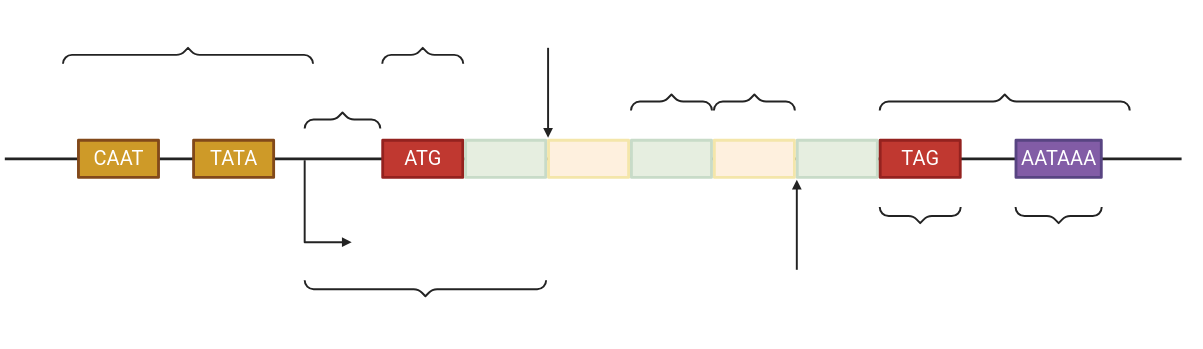
\includegraphics[width=\linewidth]{images/eukgenblank.png}
\testhead{Skizzieren sie einen BAC-Vektor}%5 
\newline \newline \newline \newline  \newline \newline 
\testhead{Zeichnen Sie das tn5 Transposon (detailliert)}%prak
\newline \newline \newline \newline  \newline \newline 
\testhead{Zeichne ein IS-Element}%prak
\newline \newline \newline \newline  \newline \newline 
\head{Beschriften eines Antikörpers}
\head{Blunt und sticky ends einzeichnen}
\testhead{Skizzieren Sie den Ablauf eines Proteinversuchs von der Zellkultur bis zur Auswertung} \newline \newline \newline \newline  \newline \newline 

\section{Multiple Choice}
\head{Was ist der Tanspositionsmechanismus von Tn5? (1 Antowort)}%prak
\begin{itemize}
    \item[[ ]] □ konservativ
\item[[ ]] □ multiplikativ
\item[[ ]] □ transpositiv
\item[[ ]] □ replikativ
\end{itemize}

\head{Welche der folgenden Eigenschaften hat ein suicide-Vektor}%prak
\begin{itemize}
    \item[[ ]] □ Transposon
    \item[[ ]] □ Breiter Wirtsbereich
    \item[[ ]] □ IS-Element
    \item[[ ]] □ Eingeschr¨ankter Wirtsbereich
    \item[[ ]] □ Mutator
    \item[[ ]] □ oriT
\end{itemize}

\head{title=Welche der folgenden Eigenschaften hat ein IS-Element}%prak
\begin{itemize}
    \item[[ ]] □ suicide
    \item[[ ]] □ IR
    \item[[ ]] □ Replikase
    \item[[ ]] □ Transponase
    \item[[ ]] □ broad host range
    \item[[ ]] □ repeats
\end{itemize}

\section{Beispiele}
\head{3 Beispiele von epigenetischen Modifikationen an Histonen}%3
\begin{itemize}
    \item 
    \item 
    \item 
\end{itemize}
\head{3 NAPs}%3
\begin{itemize}
    \item 
    \item 
    \item 
\end{itemize}
\head{Nenne Sie drei verschiedene Inonisierungsmethoden}%11
\head{Bennen Sie die drei (Sub)Genome einer eukaryotischen Zelle}%3
\begin{itemize}
    \item 
    \item 
    \item 
\end{itemize}
\head{3 Techniken, um Genexpression zu messen/untersuchen}%9
\begin{itemize}
    \item 
    \item 
    \item 
\end{itemize}
\head{Bestandteile des Massenspektrometers}%11
\begin{itemize}
    \item 
    \item 
    \item 
\end{itemize}
\testhead{Reaktionskomponenten der PCR und deren ungefähre Temperaturen} \newline  \newline \newline 
\head{Nennen Sie die drei wichtigsten Komponenten der Klonierung und ihre Funktion.}%2
\begin{itemize}
    \item 
    \item 
    \item 
\end{itemize}
\head{Nennen sie zwei Beispiele für large insert clone Vektoren}%5
\begin{itemize}
    \item 
    \item 
\end{itemize}
\head{3 versch. Techniken zum Messen des Expressionszustand von Genen + deren wesentliche Eigenschaften}%9
\begin{itemize}
    \item 
    \item 
    \item 
\end{itemize}

\begin{figure}[H]
    \centering
    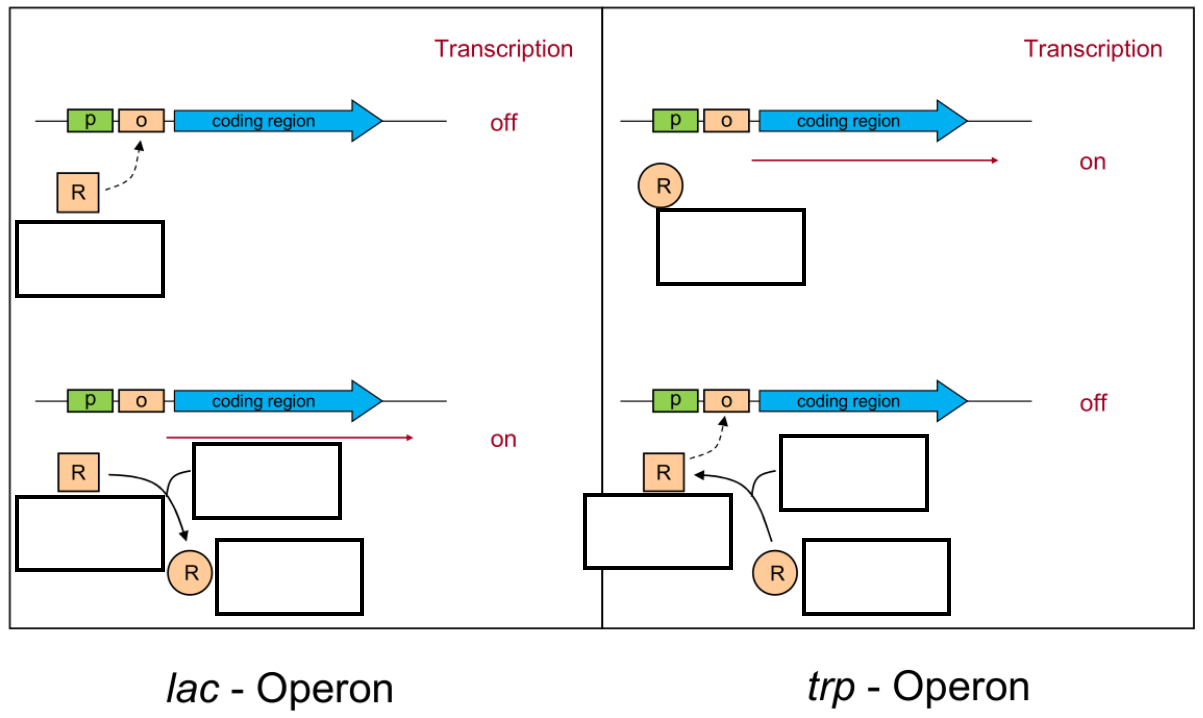
\includegraphics[width=12cm]{images/repressorbildblank.png}%prak
\end{figure}
